\chapter{فعالیت‌ها و تجربیات کارآموزی}

در این قسمت به تجربیات کسب شده در دوره کارآموزی شرکت عصر‌گویش‌پرداز پرداخته خواهد شد. در این دوره کارآموزی، در سه پروژه بازشناسی گفتار به واسطه صوت و تصویر (پرشین ای-وی-اس-آر
\LTRfootnote{PersianAVSR}
)، اصلاح گرامری و نحوی متن (کاتب 
\LTRfootnote{Kateb}
) و اصلاح نشانه‌گذاری متن
\LTRfootnote{Punctuation} 
خروجی مدل بازشناسی گفتار (کاتب ای-اس-آر
\LTRfootnote{Kateb-ASR}
) فعالیت داشته‌ام. در ادامه، فعالیت‌های انجام شده در هر یک از پروژه‌ها به تفصیل بیان خواهد شد.

\section{پروژه پرشین ای-وی-اس-آر}

در این بخش، در ابتدا به صورت خلاصه مساله و ضرورت حل آن بررسی خواهد شد سپس به بررسی فعالیت‌های انجام شده در جهت حل این مساله و آماده‌سازی یک خدمت
\LTRfootnote{Service}
برای ارائه آن، پرداخته خواهد شد.

\subsection{مساله بازشناسی گفتار}

مهم‌ترین راه ارتباطی انسان، زبان و یکی از ارکان مهم آن، گفتار می‌باشد. بنابراین یکی از مناسب ترین روش‌ها برای ارتباط و تعامل با رایانه‌ها، گفتار می‌باشد. به همین دلیل این مساله، یکی از مهم‌ترین مسائل عصر حاضر می‌باشد. 

رویکرد غالب در جهت حل این مساله، ایجاد سامانه‌ای است که با دریافت گفتار به صورت سیگنال‌های صوتی، آن را درک کند و سپس متن متناظر با گفتار را به عنوان خروجی، برگرداند. این رویکرد، عملکرد مناسبی در موقعیت‌های بدون نویز از خود نشان می‌دهد اما در صورت قرارگیری در محیط‌ها و موقعیت‌های نویزی، دچار افت کیفیت شده و عملکرد ضعیفی از خود نشان می‌دهند.

برای حل این مساله دو رویکرد عمده وجود دارد:
\begin{itemize}
	\item تقویت گفتار
	\LTRfootnote{Speech Enhancement (SE)}
	\item بازشناسی گفتار با استفاده از ترکیب داده‌های صوتی و بصری
	\LTRfootnote{Audio-Visual Speech Recognition (AVSR)}
\end{itemize}

در این پروژه، برای افزایش پایداری
\LTRfootnote{Robustness}
مدل های بازشناسی گفتار در محیط‌های نویزی، از رویکرد دوم استفاده شده است. در این رویکرد، مدل تلاش می‌کند با استفاده از داده‌های بصری - به خصوص حرکت لب‌های فرد گوینده - ضعف قسمت‌های نویزی سیگنال‌های صوتی را جبران کرده و عملکرد بهتری از خود نشان دهد.

\subsection{بررسی پیشینه}

اولین گام در این دوره کارآموزی، مرور سوابق پژوهشی در جهت حل این مساله بوده است. برای یافتن مقالات مربوط به این مساله، با استفاده از سایت پیپرزویدکد
\LTRfootnote{Papers With Code (https://paperswithcode.com)}
، گوگل اسکولار
\LTRfootnote{Google Scholar (https://scholar.google.com)}
و کانکتدپیپرز
\LTRfootnote{Connected Papers (https://connectedpapers.com)}
فرایند جستجو مقالات را آغاز کرده و در نهایت مقالات مرتبط را با در نظر گرفتن پارامتر‌های زمان انتشار، وجود پیاده‌سازی در سایت گیت‌هاب
\LTRfootnote{Github (https://github.com)}
 و وجود مدل‌های آماده، جمع‌آوری و در یک برگه گوگل ذخیره کردم. لیست مقالات جمع‌آوری شده، در پیوست قابل مشاهده می‌باشد. % در ادامه لیبل پیوست یک اضافه شود.
 
پس از جمع‌آوری تمام مقالات، برای یافتن مقاله مناسب، به بررسی تمام مقالات پرداختم. در کل، یازده مقاله جمع‌آوری شده، دارای پیاده سازی با استفاده از چارچوب‌های
\LTRfootnote{Framework}
 تنسورفلو
\LTRfootnote{Tensorflow}
و پایتورچ
\LTRfootnote{PyTorch}
بودند. از میان این یازده مقاله، به دلیل جدیدتر بودن، وجود پیاده‌سازی در گیت‌هاب و وجود مدل های آماده، مدل ای-وی هیوبرت
\LTRfootnote{Audio-Visual HuBERT (AV-HuBERT)}
 و مقاله مربوط به آن
\LTRfootnote{Robust Self-Supervised Audio-Visual Speech Recognition (https://arxiv.org/abs/2201.01763)}
را انتخاب نمودم.

\subsection{مدل خود-نظارتی ای-وی هیوبرت}

مدل ای-وی هیوبرت، یک مدل خود-نظارتی
\LTRfootnote{Self-Supervised}
می‌باشد و آموزش آن شامل دو مرحله پیش‌آموزش بر روی داده‌های بدون برچسب و کوک کردن آن با استفاده از داده‌های برچسب‌گذاری شده می‌باشد. به همین دلیل، این مدل با استفاده با حجم کم‌تری از داده‌های برچسب‌گذاری شده، عملکرد بهتری نسبت به مدل های نظارت‌شده
\LTRfootnote{Supervised}
 از خود نشان می‌دهد.

ساختار یادگیری این مدل، از رویکرد اصلی آموزش در مدل زبانی معروف برت
\LTRfootnote{Bidirectional Encoder Representations from Transformers (BERT)}
 الهام گرفته شده است. مدل زبانی برت، یک مدل مبتنی بر ترنسفورمر
 \LTRfootnote{Transformer}
  می‌باشد و برای یادگیری سعی می‌کند قسمتی از جمله ورودی - برای مثال تعدادی از کلمات موجود در جمله - را پوشانده و در ادامه با کمک کلمات مجاور و ساختار جمله، کلمات پوشانده شده را حدس بزند. این روش منجر می‌شود با حجم داده برچسب‌گذاری شده کمتر و داده‌های بدون برچسب، مدل درک مناسبی نسبت به ساختار جملات و جایگاه کلمات در جمله به دست آورد. 

با الهام از این ایده، مدل هیوبرت
\LTRfootnote{HuBERT}
برای حل مساله بازشناسی گفتار به واسطه صوت
\LTRfootnote{Automatic Speech Recognition}
پیشنهاد شده است. یکی از تفاوت های اساسی حوزه صوت و متن، ساختار داده ورودی می‌باشد. در حوزه متن، ورودی‌ها به دلیل گسسته بودن، قابل شکستن به ساختار‌های کوچک‌تر با معنی به صورت توکن
\LTRfootnote{token}
یا کلمات می‌باشند در صورتی که صوت،دارای ماهیت پیوسته بوده و به همین دلیل به طور مستقیم چنین امکانی در این حوزه وجود ندارد. برای حل این مشکل و گسسته سازی صوت و گفتار، پژوهشگران از آوا‌ها و هجاها به عنوان کوچکترین ساختار‌های معنی‌دار در این حوزه استفاده کرده و گفتار را به صورت ترکیبی از آنها تعریف کردند. 

در این مدل، برای استخراج آوا‌ها، از استخراج‌کننده ویژگی
\LTRfootnote{Feature Extractor}
ام-اف-سی-سی
\LTRfootnote{Mel-Frequency cepstrum coefficients (MFCC)}
استفاده شده است. این استخراج‌کننده ویژگی با دریافت گفتار، ویژگی‌های با ابعاد ۳۹ را در هر لحظه تولید می‌کند. در نهایت با یک الگوریتم خوشه‌بندی نظیر کا-مینز
\LTRfootnote{K-means}
آواهای اصلی مشخص شده و در فرایند آموزش به عنوان واحد‌های سازنده گفتار، شرکت می‌کنند. فرایند استخراج ویژگی، تنها در دور
\LTRfootnote{Epoch}
اول به واسطه استخراج‌کننده ویژگی ام-اف-سی-سی انجام شده و در مراحل بعدی به واسطه بازنمایی موجود در لایه‌های میانی شبکه کد‌کننده
\LTRfootnote{Encoder}
ترنسفورمر انجام می‌شود.

در ادامه برای یادگیری مدل، بخشی از آواها و هجاهای اصلی که در فرایند خوشه‌بندی مشخص شده‌اند، در گفتار ورودی پوشانده شده و مدل تلاش می‌کند تا با توجه به ارتباط میان آواها و یادگیری ساختار آنها، بخش پوشانده را حدس بزند. در این روش، از تابع خطا آنتروپی متقاطع
\LTRfootnote{Cross Entropy}
و الگوریتم‌های بهینه‌سازی نظیر الگوریتم آدام
\LTRfootnote{Adam}
استفاده شده است.

\begin{figure}[!h]
	\centering
	\captionsetup{justification=centering}
	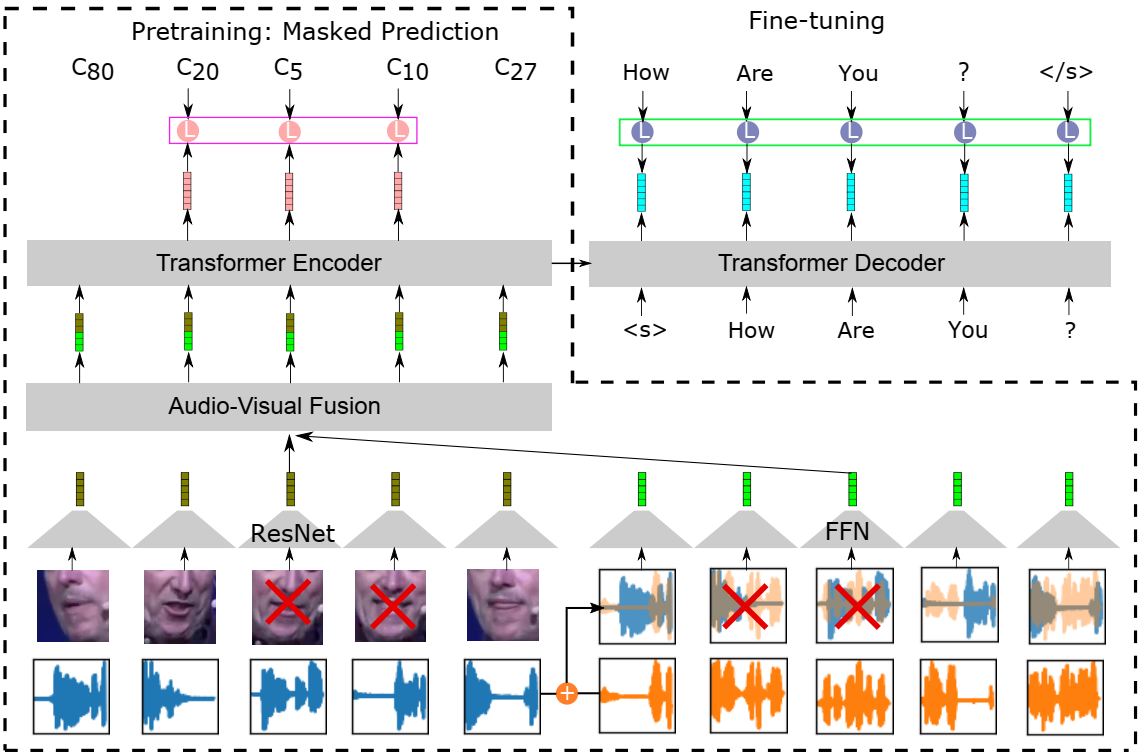
\includegraphics[width=\textwidth]{images/av-hubert-model}
	\caption[معماری مدل ای-وی هیوبرت]{معماری مدل ای-وی هیوبرت \cite{shi2022robust}}
	\label{fig:av-hubert-model}
\end{figure}

مدل ای-وی هیوبرت، بر پایه مدل هیوبرت ارائه شده است و رویکردی مشابه را این‌بار برای حل مساله بازشناسی گفتار به واسطه صوت و تصویر در پی می‌گیرد. همانطور که در تصویر 
\ref{fig:av-hubert-model}
مشاهده می‌شود، در این مدل فریم‌های صوتی و بصری ویدیو، به ترتیب به واسطه کدکننده صوتی و کدکننده بصری به یک بازنمایی متراکم
\LTRfootnote{Dense Representation}
تبدیل می‌شوند.

در کدکننده بصری، از یک مدل رزنت-هجده 
\LTRfootnote{ResNet-18}
شده است. مدل های رزنت، به جای ساختار ترتیبی لایه‌ها، دارای اتصالات خارج از ترتیب بوده که موجب کاهش مشکل محوشدن گرادیان
\LTRfootnote{Vanishing Gradient}
و به تبع آن، افزایش تعداد لایه‌های مدل می‌شود. این نوع از مدل‌ها، پیش از ارائه مدل‌های مبتنی بر ویژن‌ترنسفورمر
\LTRfootnote{Vision Transformer (ViT)}
، دارای بهترین عملکرد در حوزه تصویر بوده‌اند. پیش از ورودی دادن فریم‌های بصری ویدیو به این مدل رزنت-هجده، تغییرات زیر بر روی تصویر اعمال می شود.

\begin{itemize}
	\item ۶۸ نقطه کلیدی چهره تشخیص داده شده و سپس به واسطه یک تبدیل خطی، این نقاط کلیدی به یک دستگاه مختصات متمرکز بر چهره انتقال پیدا می‌کند.
	\item یک منطقه مورد علاقه
	\LTRfootnote{Region of Interest (ROI)}
	با ابعاد ۹۶×۹۶ حول دهان فرد در چهره بریده می‌شود.
	\item کانال‌های رنگی تصویر به سطح خاکستری منتقل می‌شوند.
	\item در جهت داده‌افزایی
	\LTRfootnote{Data Augmentation}
	یک کادر با ابعاد ۸۸×۸۸ به صورت تصادفی از منطقه مورد علاقه بریده شده و به صورت تصادفی به صورت افقی قرینه
	\LTRfootnote{Horizontal Flip}
	می شود.
\end{itemize}

به دلیل تاثیر بیشتر داده‌های صوتی نسبت به داده‌های بصری در این مساله، برای کاهش تاثیر داده‌های صوتی و افزایش تاثیر داده‌های بصری در یادگیری مدل، از یک شبکه تماما متصل عصبی استفاده شده است. فریم‌های صوتی خام ورودی، پیش از ورودی داده شدن به شبکه عصبی، به واسطه یک استخراج کننده ویژگی خاص
\LTRfootnote{Log Filterbank Energy}
به یک بردار ۲۶ بعدی با فاصله ۱۰ میلی‌ثانیه تبدیل می‌شود. علاوه بر این، به دلیل تفاوت نرخ برداشت فریم های صوتی و بصری - فریم‌های صوتی با فرکانس صد هرتز و فریم‌های بصری با فرکانس ۲۵ هرتز برداشت می‌شود - به ازای هر فریم بصری،چهار فریم صوتی برداشت می‌شود تا هماهنگی زمانی میان دو نوع داده حفظ شود.

\section{پروژه کاتب}

\section{پروژه کاتب ای-اس-آر}